\chapter{Webapplikation Angular}
\label{chp:frontend}

Der Prototyp verfügt über eine verlässliche, schnelle Webapplikation, welche mit Angular entwickelt worden ist. \emph{Angular} ist ein von Google entwickeltes Framework zur einfachen Erstellung von skalierbaren und performanten Webapplikationen. Die Erlernung der Grundlagen des Frameworks ist im Vergleich zu anderen JavaScript-Frameworks deutlich einfacher. Die Grundprinzipien umfassen das Verständnis eines Komponenten, das Routing von Angular bei einer Single Page Application und Dependency Injection im Allgemeinen. Da die detaillierten Funktionalität von Angular bereits im Architekturkapitel besprochen worden sind, gehen wir hier nicht mehr näher darauf ein. Stattdessen wird dieses Kapitel die Funktionalität unsere Webapplikation im Näheren behandeln. \cite{AngularFeatures,AngularComponents,AngularDI}

Die Angular Applikation hat eine Ordnerstruktur des in der Abbildung \ref{fig:AngularDirectoryStructurePrototype} zu sehenden Aufbaues. Wie Sie sehen können, gibt es auf Root-Ebene einige Konfigurationsdateien, darunter \wordindoublequotes{angular.json}, \wordindoublequotes{tsconfig.json} und \wordindoublequotes{nginx.conf}. Diese Dateien enthalten Basiskonfigurationen der Webapplikation, wie zum Beispiel Definitionen für bestimmte CLI Kommandos, Moduloptionen und verschiedene Entrypoints für die kompilierten HTML-Dateien. Im \wordindoublequotes{/app}-Ordner befinden sich dann die Dateien für die Komponenten. Wie Sie anhand des Ordners \wordindoublequotes{navigation} in Abbildung \ref{fig:AngularDirectoryStructurePrototype2} sehen können, besteht jeder Komponent aus HTML, Typescript, CSS und Spezifikationsdatei. Wir haben die Applikation in vier Komponenten aufgeteilt, die Navigation umschließt je nach Seite immer eine andere Komponente, entweder das Dashboard, die Tabelle oder den Graphen.

\begin{figure}
    \centering
    \begin{subfigure}{.5\textwidth}
        \centering
        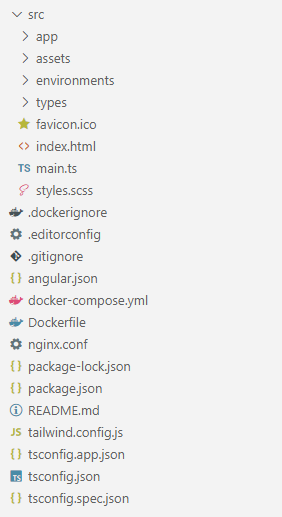
\includegraphics[width=.75\linewidth]{content/img/Empire/Frontend/Angular_Directory_Structure_Prototype_1.png}
        \caption{Ordnerstruktur Root-Ebene}
        \label{fig:AngularDirectoryStructurePrototype1}
    \end{subfigure}%
    \begin{subfigure}{.5\textwidth}
        \centering
        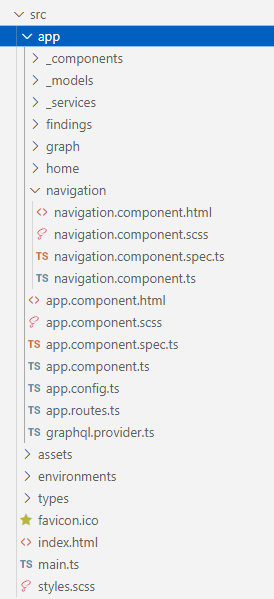
\includegraphics[width=.65\linewidth]{content/img/Empire/Frontend/Angular_Directory_Structure_Prototype_2.png}
        \caption{Ordnerstruktur des \wordindoublequotes{/src}-Ordners}
        \label{fig:AngularDirectoryStructurePrototype2}
    \end{subfigure}
    \caption{Ordnerstruktur der Webapplikation (Angular)}
    \label{fig:AngularDirectoryStructurePrototype}
\end{figure}
\FloatBarrier

Das Auffälligste bei diesem Teil des Prototypen ist die konsistente Umsetzung des Corporate Designs von Siemens. Die ikonische türkise -- manche Menschen würden auch einfach blau oder grün dazu sagen -- Unternehmensfarbe zieht sich dank Angular Theme durch die gesamte Webapplikation. Angefangen beim Logo, über die Anwendungsleiste am oberen Bildschirmrand bis hin zu den Ladebalken und ähnlichem ist alles in dem typischen Siemens-Türkis gehalten. Diese Entscheidung ist bewusst getroffen worden, da die Farbe sofort auf das Unternehmen selbst referenziert. Einen Teil dieses Designs dürfen Sie in Abbildung \ref{fig:AngularSneakPeak} genießen.

\begin{figure}
    \centering
    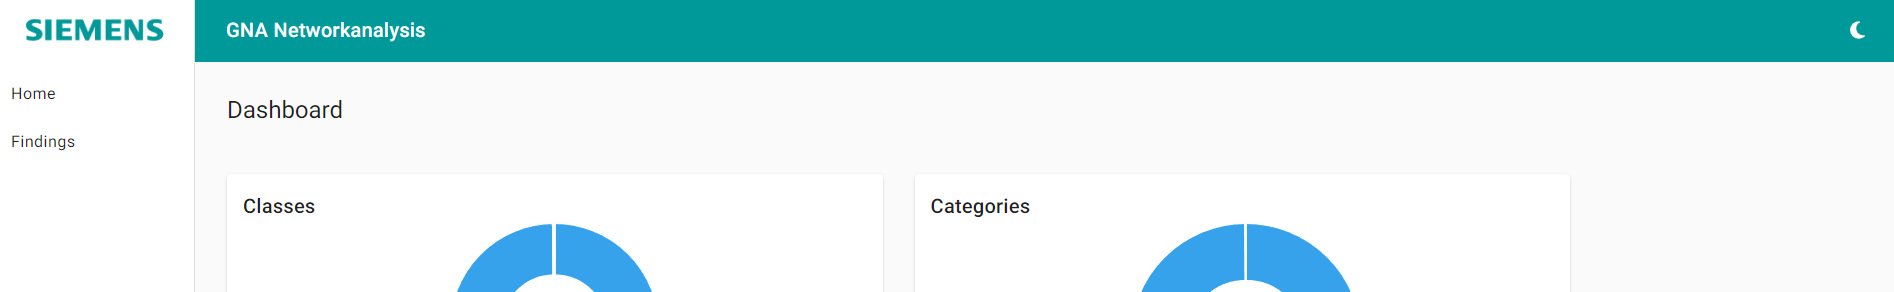
\includegraphics[width=1\textwidth]{content/img/Empire/Frontend/Angular_Sneak_Peak.png}
    \caption{Sneak Peak unserer Angular Applikation}
    \label{fig:AngularSneakPeak}
\end{figure}
\FloatBarrier

\faInfoCircle\hspace{2mm}In der Entwicklungsphase des Prototypen sind anonymisierte Testdaten verwendet worden, da Clemens und Felix rechtlich gesehen keine Kundendaten sehen dürfen.

\section{Dashboard mit Kennzahlen des Netzmodells}
\label{chp:dashboard}

\setcapindent{0pt}
\begin{wrapfigure}{r}{0.27\textwidth}
  \begin{center}
    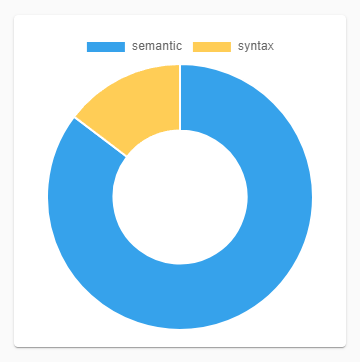
\includegraphics[width=0.8\linewidth]{content/img/Empire/Frontend/Dashboard_Donatdiagramm.png}
  \end{center}
  \caption{Donatdiagramm}
  \label{fig:einfachesDonatdiagramm}
\end{wrapfigure}
\setcapindent{83pt}

Kennzahlen in einem Dashboard attraktiv, benutzerfreundlich und intuitiv darzustellen, ist selbst für fortgeschrittene Designer oft ein langwieriger Prozess. Eine einfache Art, die Dauer für die Schaffung eines übersichtlichen Dashboardes zu minimieren, ist die Verwendung von vorgefertigten UI-Elementen. Diese Elemente können aus beliebigen Bibliotheken stammen. Für Angular eignet sich am besten die Bibliothek \emph{ng2-charts}.

In der Abbildung \ref{fig:einfachesDonatdiagramm} rechts ist ein Beispiel eines Donatdiagrammes mittels ng2-charts gegeben. Dieses wird im Dashboard verwendet, um die Verteilung der beiden Kategorien darzustellen.

Die Bibliothek ng2-charts ist im Prinzip eine Schnittstelle zwischen Angular und einer universellen Javascript-Diagramm-Bibliothek namens \emph{Chart.js}. Diese unterstützt wiederum eine Vielzahl an Diagrammen, von Linien- über Flächen bis hin zu Donatdiagrammen. Für das Dashboard unseres Netzwerkanalyseprogrammes habe ich ausschließlich Donatdiagramme verwendet, um die prozentuellen Verteilungen der verschiedenen Eigenschaften, darunter der Schweregrad, die Kategorie, das Spannungslevel und die Klasse beziehungsweise der Typ des Fehlers, einheitlich darzustellen. \cite{ng2-charts}

Diese Bibliothek wird nun verwendet, um vier Donatdiagramme auf dem Dashboard darzustellen. Diese Diagramme geben den Ingenieuren von Siemens einen schnellen Überblick über grundlegende Eigenschaften der aktuellen Fehler im Netzmodell. Jedes der vier Diagramme stellt die prozentuelle Verteilung bezüglich einer Eigenschaft dar. Diese vier Eigenschaften sind: Klasse, Kategorie, Schweregrad und Spannungslevel. Wie Sie in Abbildung \ref{fig:PrototypeDashboard} sehen können, sind alle vier Eigenschaften sehr einseitig. Mit dieser Einseitigkeit ist die klare Dominanz beziehungsweise die Vorherrschaft des Hauptsegmentes der jeweiligen Eigenschaft gemeint. An den Legenden können Sie sehen, dass beispielsweise fast alle Fehler im Netzmodell mit Schweregrad \wordindoublequotes{CRITICAL} kategorisiert worden sind (der große gelbe Anteil im dritten Diagramm in Abbildung \ref{fig:PrototypeDashboard}).

\begin{figure}
    \centering
    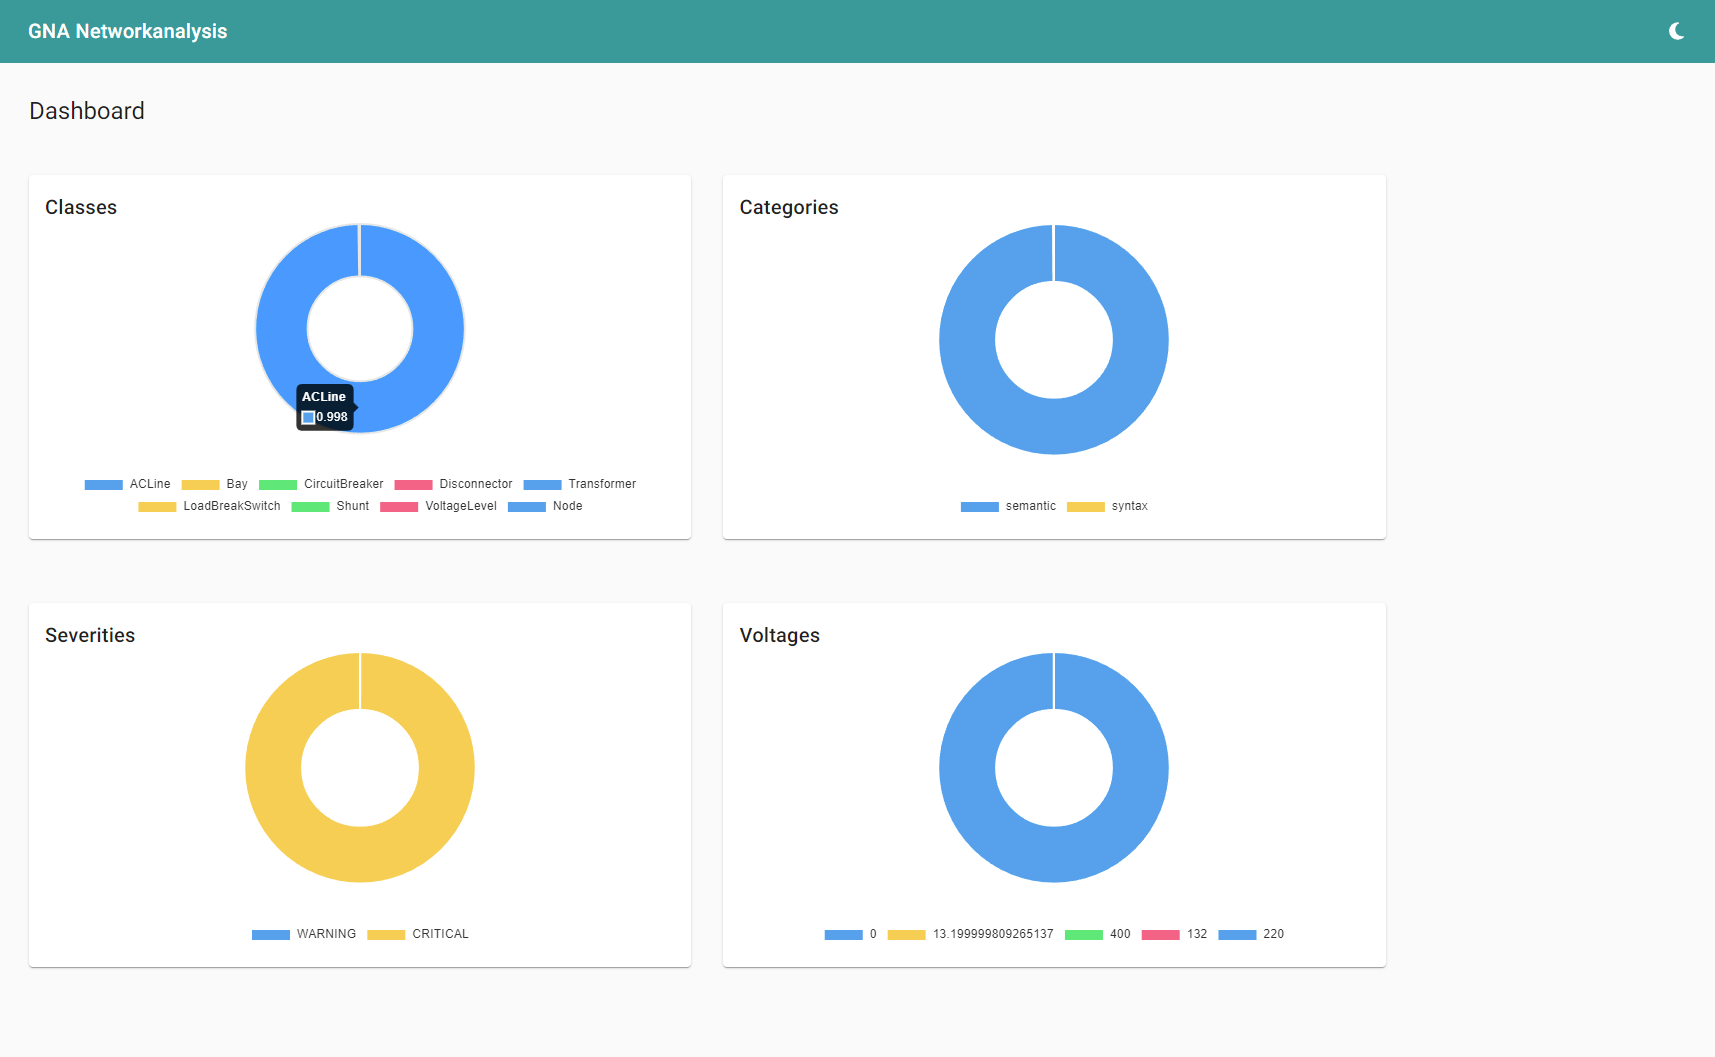
\includegraphics[width=1\textwidth]{content/img/Empire/Frontend/Angular_Dashboard_Prototype.png}
    \caption{Dashboard des Prototypen}
    \label{fig:PrototypeDashboard}
\end{figure}
\FloatBarrier

Bei diesen Diagrammen wird auch ein hoher Wert auf die Interaktivität gelegt. Wie Sie beim ersten Diagramm in Abbildung \ref{fig:PrototypeDashboard} auch sehen können, gibt es eine dem Mauszeiger folgende Informationen bezüglich des Anteils dieses ausgewählten Segments. Dieser sogenannte \wordindoublequotes{Tooltip} ist äußerst intuitiv, da er heutzutage schon an vielen Stellen in der Webentwicklung auftritt. \cite{chartjs-interactions}

Um die Interaktivität noch mehr zu steigern, ist bei Chart.js standardmäßig auch die Funktion implementiert, bestimmte Anteile im Diagramm dynamisch auszublenden. Bei schlauem Anwenden dieser Funktion, können bereits sehr nützliche Informationen aus einigen Diagrammen abgelesen werden, wie Sie in Abbildung \ref{fig:PrototypeDashboardInteraction} sehen. Sie sehen zum Beispiel, dass ein Großteil der gefilterten Fehler bei Stromkreisunterbrechern und Knoten entsteht (Diagramm 1) und nur sehr wenige Fehler eine Spannung von 400V aufweisen. \cite{chartjs-legend}

\begin{figure}
    \centering
    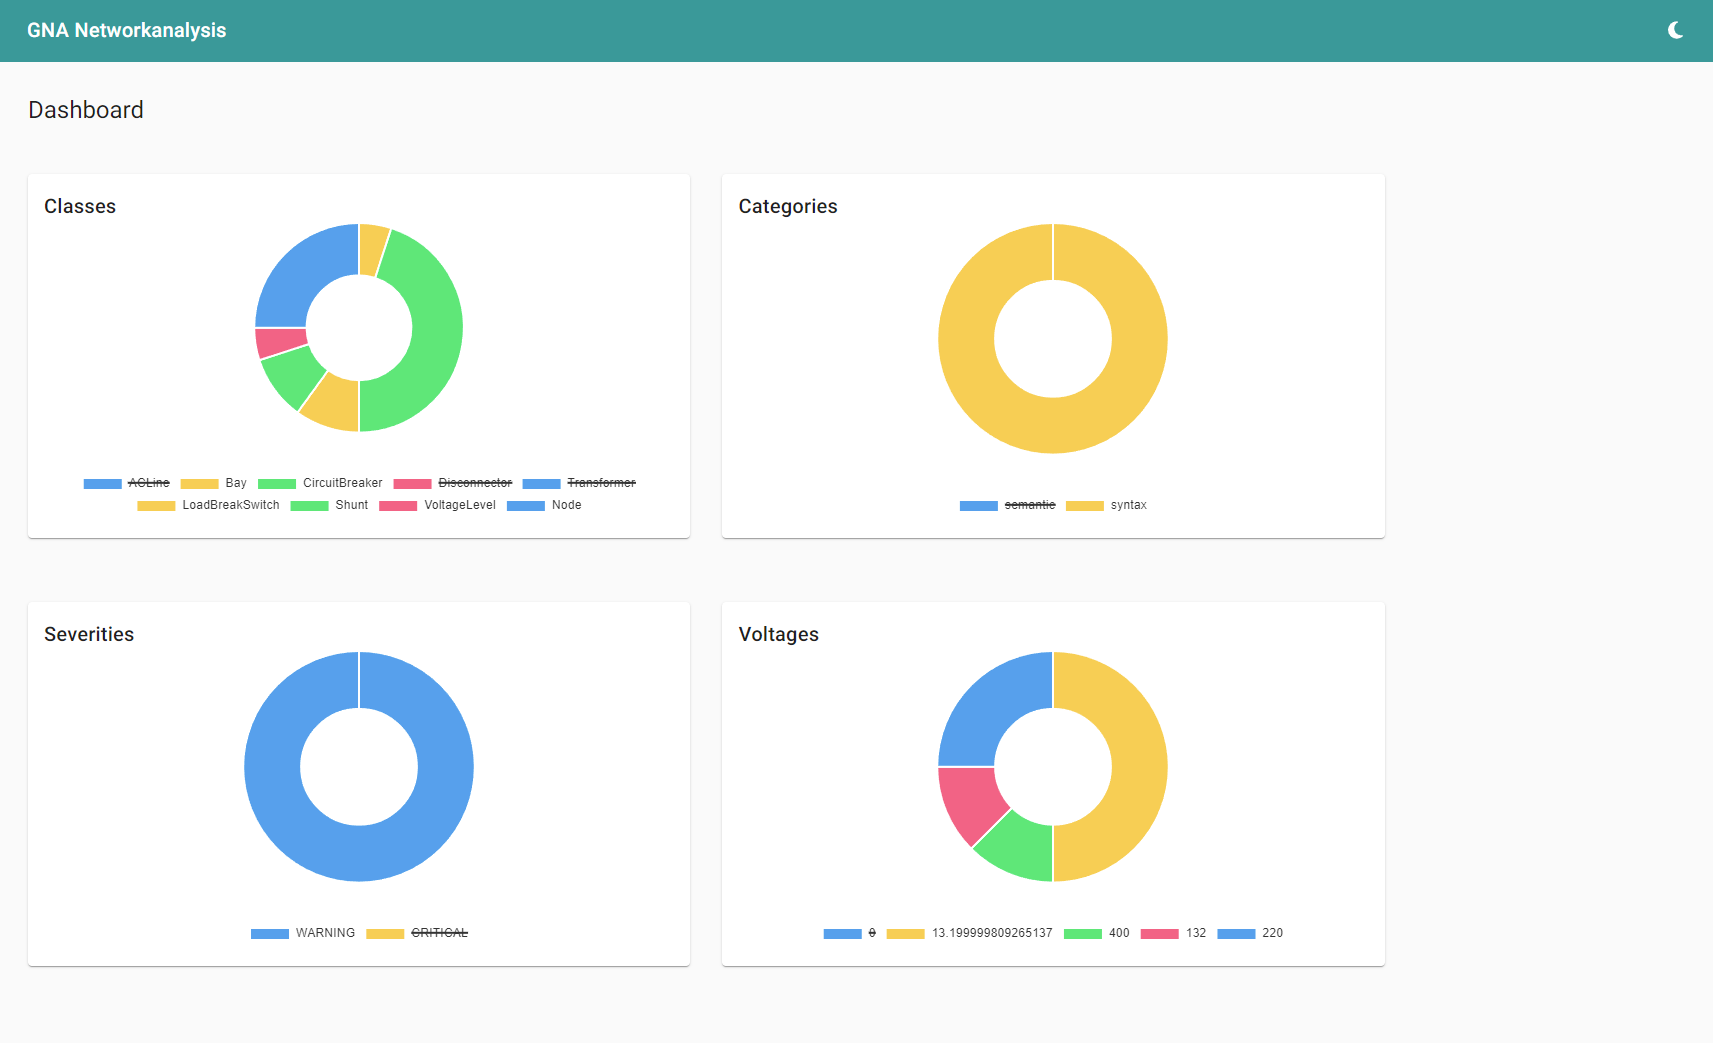
\includegraphics[width=1\textwidth]{content/img/Empire/Frontend/Angular_Dashboard_Interaction_Prototype.png}
    \caption{Interaktion mit den Diagrammen des Dashboardes}
    \label{fig:PrototypeDashboardInteraction}
\end{figure}
\FloatBarrier

Summa summarum ist das Dashboard ein sehr effizienter Weg, um einen schnellen Überblick über das aktuelle Geschehen im Netzmodell zu erhalten und bestimmte Eigenschaften im allgemeinen Kontext zu interpretieren. Die Diagramme sind intuitiv zu lesen und mit einigen Interaktionen ausgestattet. Außerdem ist das Dashboard eine wichtige Komponente moderner Applikationen, da diese immer eine Art Landingpage beziehungsweise Einstiegsseite für die Benutzer ist und diesen herzlich willkommen heißt.
\section{Tabellen mit Filter- und Suchfunktionen}

Die Applikation verfügt neben dem Dashboard auch über eine Tabelle mit Filter-, Such- und Sortierungsmöglichkeiten. Im Prinzip ist diese Tabelle eine verbesserte Darstellung der von Siemens verwendeten Log-Dateien, da interaktiv mit den Ergebnissen gearbeitet werden kann. Sie zeigt standardmäßig alle gefundenen Fehler im Netzmodell an. Dieser Fehler beziehen sich beispielsweise auf kaputte Schalter, Generatoren oder Leitungen. Allerdings können Fehler auch eine größere Bedeutung im Stromnetzwerk, wie zum Beispiel ein Umspannwerk oder eine Gruppe von Elementen, beinhalten. Mithilfe der Filtermöglichkeiten können somit schwerwiegende Fehler schneller gefunden werden. Dazu kommen wir jedoch später noch. Zuerst sehen wir uns in Abbildung \ref{fig:AngularFindingsPrototype} die Standardansicht der Tabelle an.

\begin{figure}
    \centering
    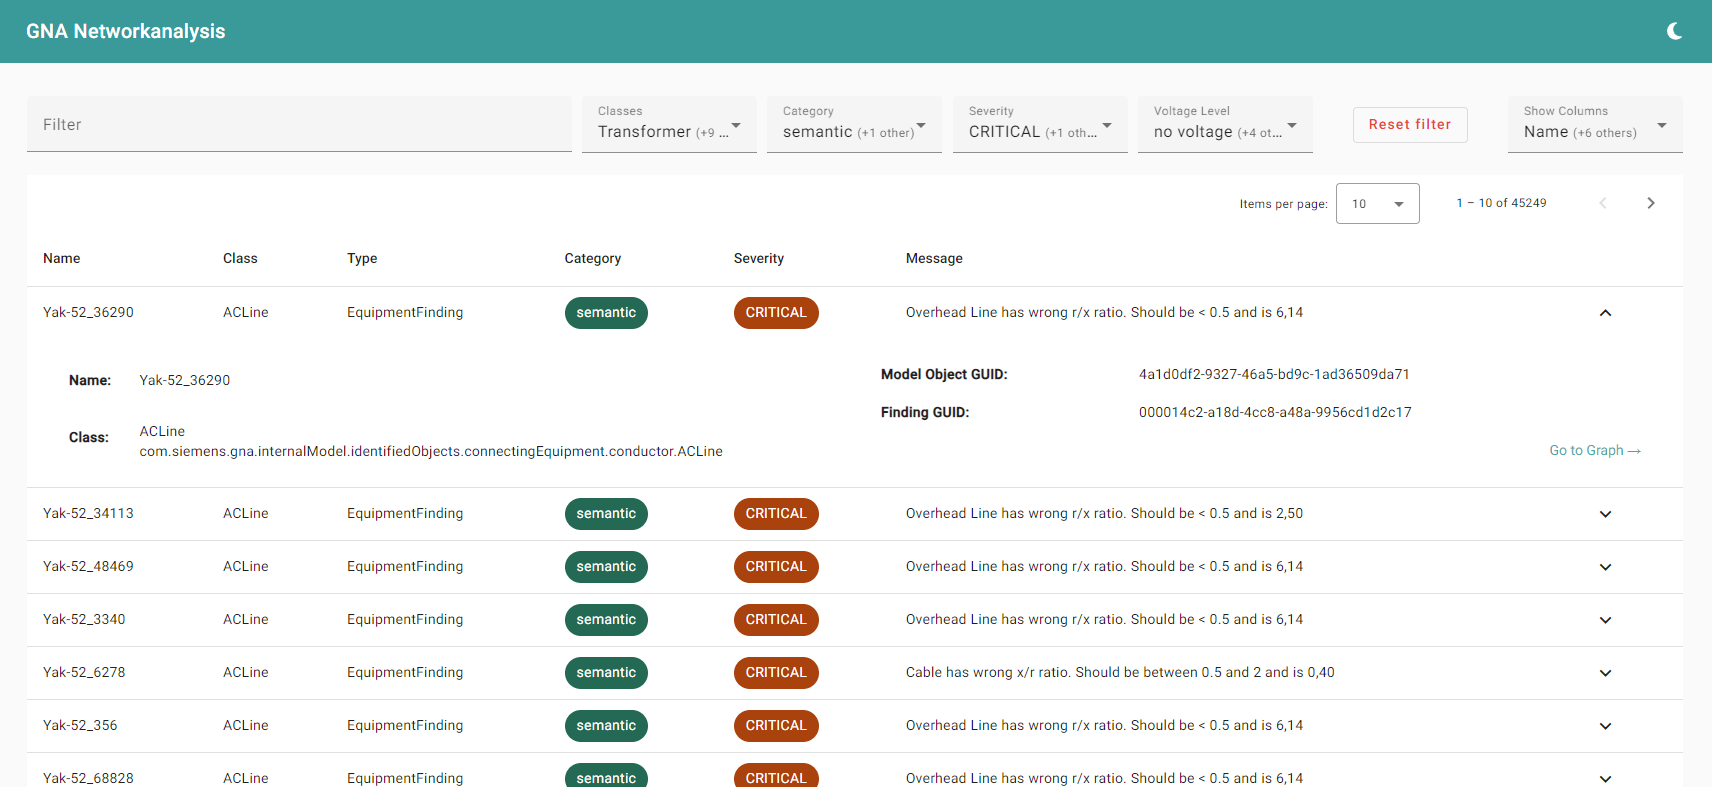
\includegraphics[width=1\textwidth]{content/img/Empire/Frontend/Angular_Findings_Prototype.png}
    \caption{Tabelle mit den aktuellen Fehlern im Stromnetzwerk}
    \label{fig:AngularFindingsPrototype}
\end{figure}
\FloatBarrier

\subsection{Sortierung}

Ein wichtiger Bestandteil moderner Tabellen in der digitalen Welt ist die Möglichkeit einer Sortierung. Diese Implementation ist dank der Bibliothek, welche in unserem Prototypen für alle UI-Elemente verwendet wird, Angular Material wirklich einfach. Nach Einstellung der Art der Sortierung -- Diese kann variieren. Beispielsweise werden bei numerischer Sortierung Zahlen logisch der Größe nach geordnet, während alphabetisches Sortieren bei Zahlen keinen Sinn ergibt, da somit \wordindoublequotes{111} vor \wordindoublequotes{22} kommen würde. -- und richtiger Handhabung der Aktualisierung der Daten, sobald eine neue Spalte ausgewählt wird, funktioniert diese wirklich verlässlich. Diese Art der Implementierung ist auch als \wordindoublequotes{deklarative Programmierung} bekannt, da man dem Framework nur sagt, \emph{was} zu tun ist. Im Gegensatz zur 
 \wordindoublequotes{imperativen Programmierung} müssen nicht die einzelnen Schritte selbst implementiert werden -- \emph{wie} etwas zu tun ist.

 In Abbildung \ref{fig:AngularFindingsSortingTypePrototype} können Sie sehen, dass die Datensätze alphabetisch aufsteigend nach dem Typen geordnet sind, wie auch an dem kleinen Pfeil neben dem Spaltennamen erkennbar ist.

\begin{figure}
    \centering
    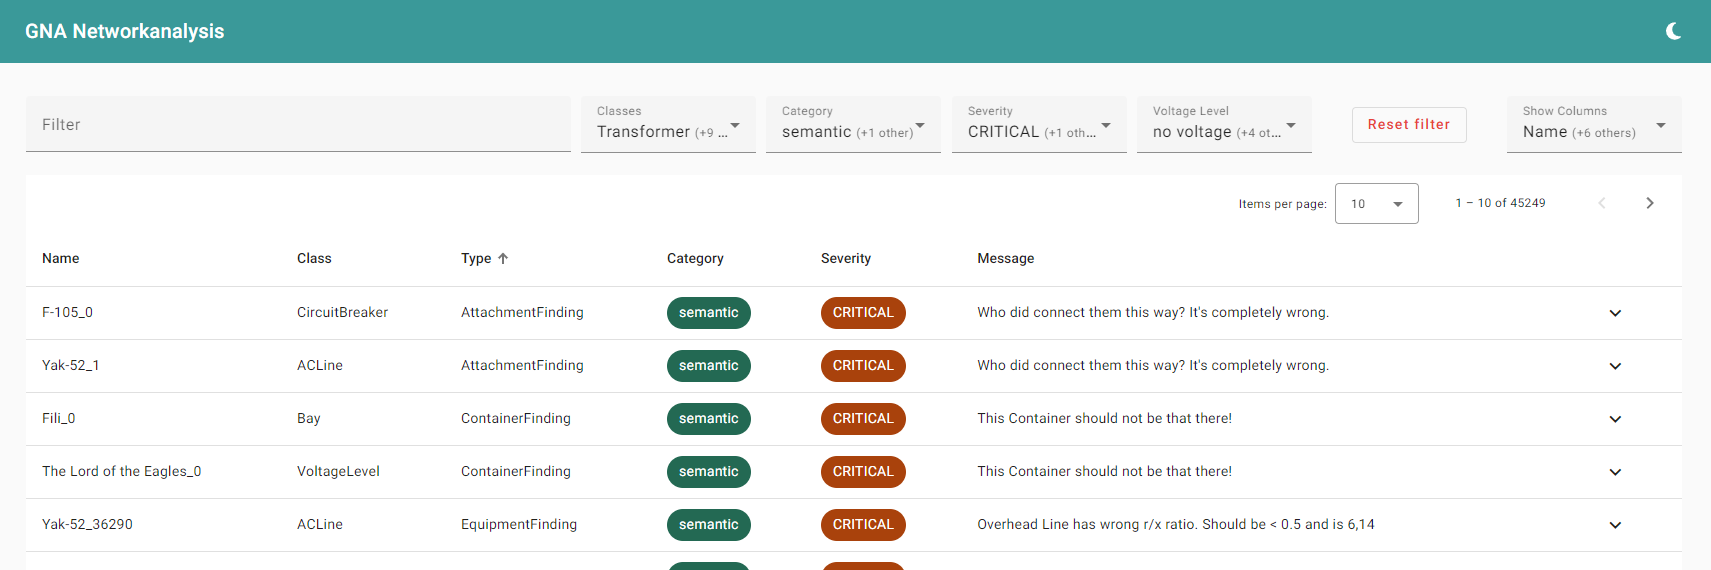
\includegraphics[width=1\textwidth]{content/img/Empire/Frontend/Angular_Findings_Sorting_Type_Prototype.png}
    \caption{Sortierungsoptionen der Tabelle des Prototypen}
    \label{fig:AngularFindingsSortingTypePrototype}
\end{figure}
\FloatBarrier

\subsection{Filterung}

Unsere Webapplikation verfügt außerdem über einige Filteroptionen. Dazu gehört natürlich ein Eingabefeld, welches über alle Spalten der Tabelle sucht und anschließend nur relevante Ergebnisse anzeigt. In Abbildung \ref{fig:AngularFindingsFilteringNodePrototype} sehen Sie beispielsweise die Filterung nach dem Wort \wordindoublequotes{Node}, welches bei den ersten drei Ergebnissen in der Klasse und ansonsten auch immer in der Nachricht des Eintrages vorkommt. Dieses Eingabefeld ist laut Siemens auch besonders wichtig, um schnell nach bestimmten Fehlern mit einer konkreten ID suchen zu können. Hierbei können Sie diese Identifikatoren zwar nicht als eigene Spalte sehen, jedoch sind sowohl die GUID des Fehlers als auch die GUID des Objektes, wo dieser Fehler im Stromnetzwerk auftritt, unter den zusätzlichen Informationen sichtbar. In Abbildung \ref{fig:AngularFindingsPrototype} haben Sie bereits diese Zusatzinformationen einsehen können.

\begin{figure}
    \centering
    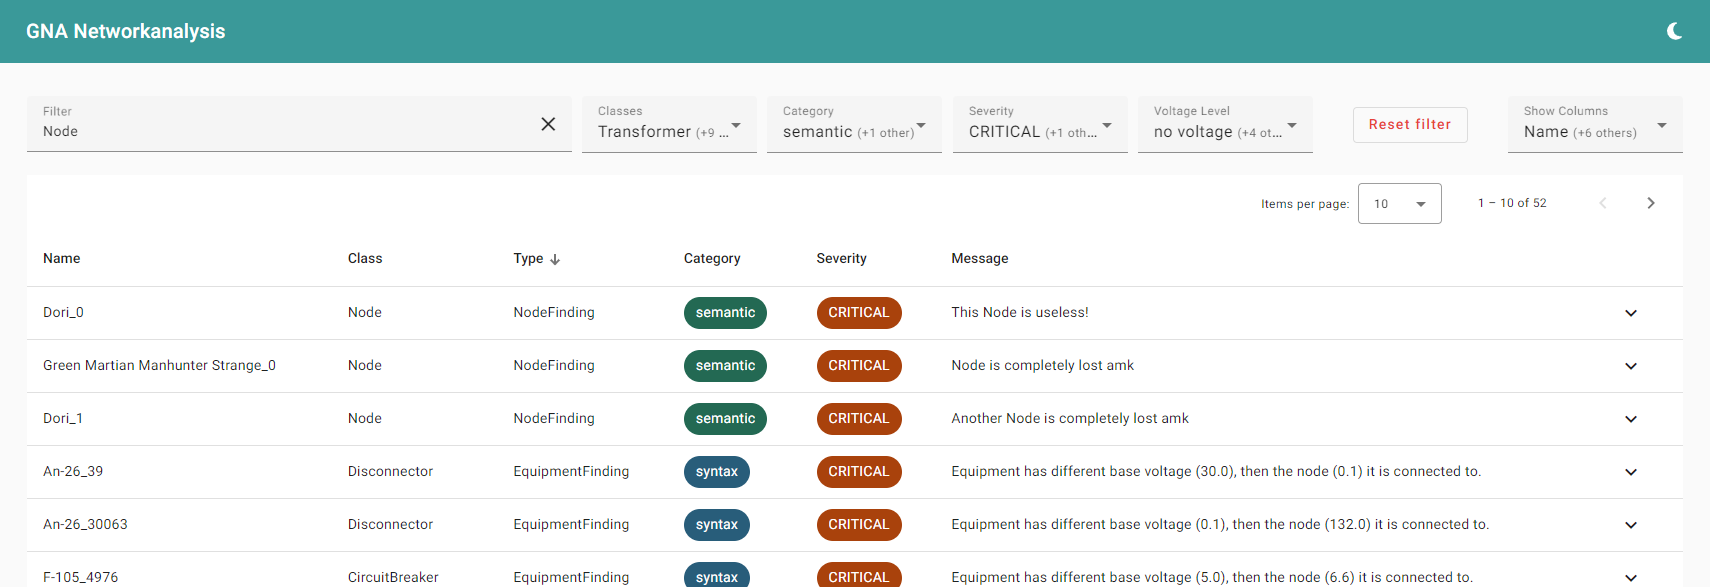
\includegraphics[width=1\textwidth]{content/img/Empire/Frontend/Angular_Findings_Filtering_Node_Prototype.png}
    \caption{Filterungsoption mit Eingabefeld über alle Spalten}
    \label{fig:AngularFindingsFilteringNodePrototype}
\end{figure}
\FloatBarrier

Im Laufe des Projektes ist noch die Anforderung hinzugekommen, die Einschränkung der Daten nach bestimmten Kriterien filter zu können. Hierbei handelt es sich genau wie beim Dashboard \ref{chp:dashboard} um die vier Eigenschaften: Klasse, Kategorie, Schweregrad und Spannungslevel. Im untigen Beispiel \ref{fig:AngularFindingsFilteringSeverityPrototype} ist die Einschränkung der Netzwerkfehler des Schweregrads abgebildet.

\begin{figure}
    \centering
    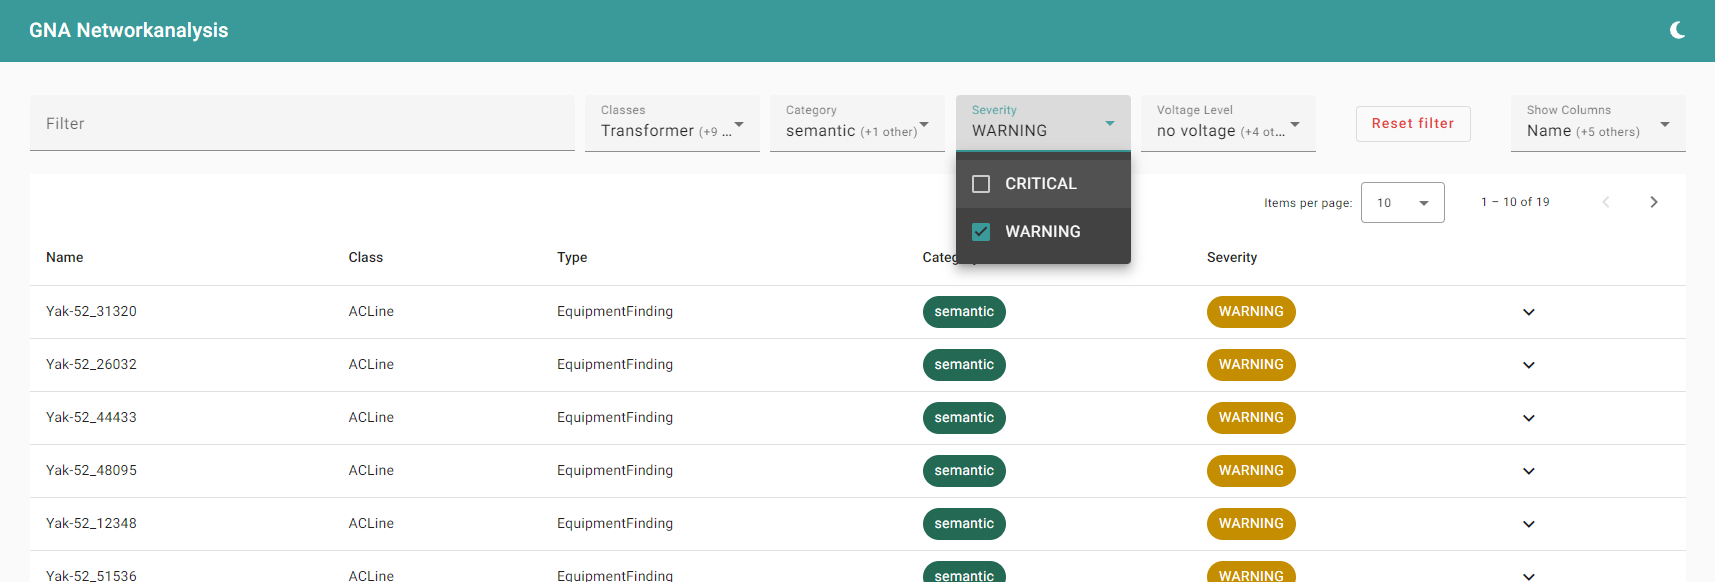
\includegraphics[width=1\textwidth]{content/img/Empire/Frontend/Angular_Findings_Filtering_Severity_Prototype.png}
    \caption{Filterungsmöglichkeit mit Dropdown-Menu für Schweregrad}
    \label{fig:AngularFindingsFilteringSeverityPrototype}
\end{figure}
\FloatBarrier

Eine wichtige Komponente der Filterungsmöglichkeiten ist der Reset-Button. Dieser erlaubt das schnelle Zurücksetzen aller Filter, falls der Benutzer das Gefühlt hat, sich in den Tiefen der Filterungsoptionen verirrt zu haben. Trotz seiner Einfachheit hat der Reset-Button in vielen Fällen eine hohe Daseinsberechtigung, da er intuitiv und äußerst nützlich ist.

\subsection{Paginierung}

Im Stromnetzwerk treten stetig einige Fehler auf, da das Netzmodell konstant umgebaut und verbessert wird. Eine \emph{GraphQL}-Abfrage, welche all diese Daten auf einmal anzeigen wollen würde, führe zwangsmäßig zu langen Ladezeiten. Aus diesem Grund hat heutzutage jeder Anwendungsfall, welcher mit vielen Daten arbeitet, irgendeine Art Pagination eingebaut. Dabei wird einfach nur ein bestimmter Teil der Daten geladen. Andere Datensätze können nach Bedarf nachgeladen werden. Während viele Social Media-Platformen auf Lazy Loading setzen -- hierbei werden neue Daten beim Scrollen nachgeladen -- verwendet unsere Applikation die von Angular Material ausimplementierte Pagination. Der Nutzer kann hierbei einfach auf die beiden Pfeile rechts oben klicken, um weitere Einträge zu laden. Um die Orientierung über die Daten zu behalten, werden außerdem ständig Informationen bezüglich den momentan angezeigten Elementen dargestellt. Beispielsweise lässt sich der Nutzer in Abbildung \ref{fig:AngularFindingsPaginationPrototype} gerade die Elemente 351 bis 375 anzeigen. Insgesamt verfügen unsere Testdaten über 45.249 Datensätze.

\begin{figure}
    \centering
    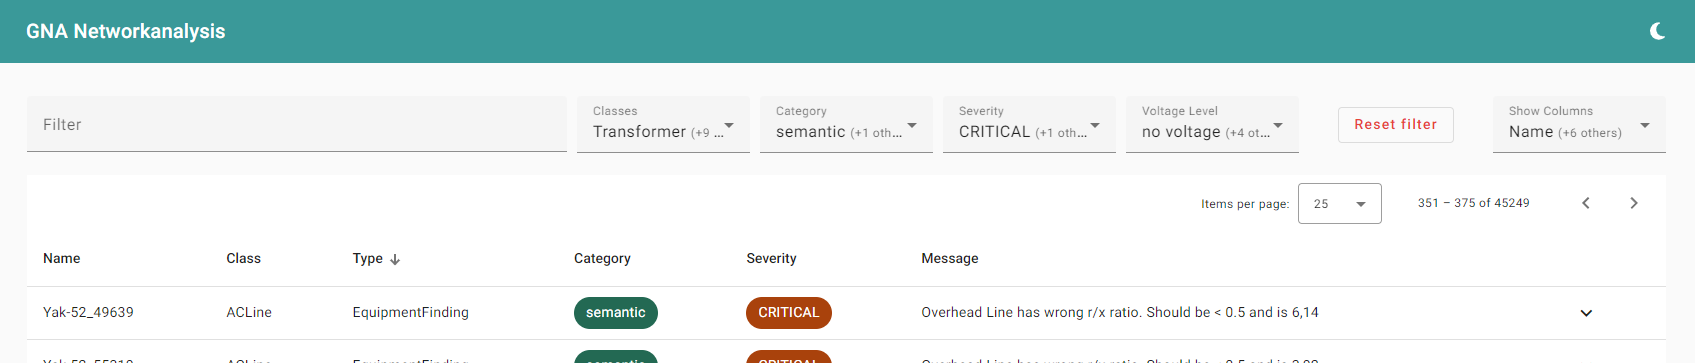
\includegraphics[width=1\textwidth]{content/img/Empire/Frontend/Angular_Findings_Pagination_Prototype.png}
    \caption{Paginierung der Tabelle mit den Fehlern}
    \label{fig:AngularFindingsPaginationPrototype}
\end{figure}
\FloatBarrier

\subsection{Besonderheit: Spannung}

Einige Datensätze verfügen über die zusätzliche Information des Spannungslevels. Dieses wird dynamisch unter den zusätzlichen Informationen angezeigt und außerdem können Sie nach diesen Werten filtern, da sie eine große Bedeutung im Stromnetzwerk haben. Aufgrund von Zeitmangel ist sich die Implementation der rekursiven Abfragen nach dem Spannungslevel nicht mehr ausgegangen. Das Netzmodell ist nämlich vereinfacht geschrieben in einer Baumstruktur aufgebaut. Teilweise haben Container höher in dieser Struktur Informationen bezüglich der Spannung des gesamten Bereiches. Jedoch hätte bei der Implementierung dieser Funktionalität die Rekursion zur Auflösung des Baummodells eine komplexere Datenabfrage zur Folge gehabt, weshalb auf dieses Feature verzichtet worden ist. Dieses Leistungsmerkmal könnte zukünftig noch erweitert werden.

Der anonymisierte Eintrag \wordindoublequotes{Giant Cyclops X\_24} in Abbildung \ref{fig:AngularFindingsVoltagePrototype} verfügt zum Beispiel über ein Spannungslevel von 220kV.

\begin{figure}
    \centering
    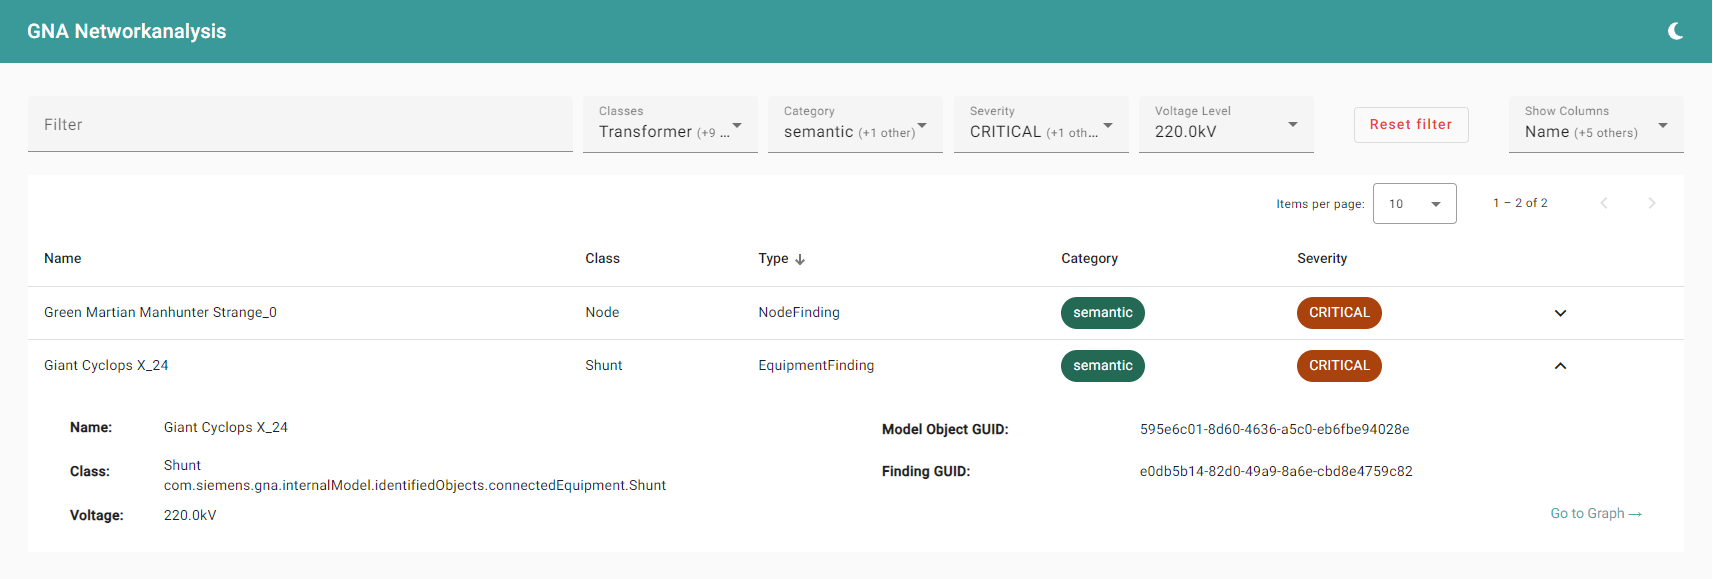
\includegraphics[width=1\textwidth]{content/img/Empire/Frontend/Angular_Findings_Voltage_Prototype.png}
    \caption{Einträge, welche über einen Spannungswert von 220.0kV verfügen}
    \label{fig:AngularFindingsVoltagePrototype}
\end{figure}
\FloatBarrier

Wie Sie in dieser Abbildung (\ref{fig:AngularFindingsVoltagePrototype}) auch schön sehen können, verfügt jeder Eintrag über einen \wordindoublequotes{Go to Graph →}-Button unten rechts. Wohin dieser den Benutzer führt, wollen wir uns als nächstes ansehen.
\section{Graph des Stromnetzmodells}

Die Visualisierung eines gesamten Stromnetzwerkes auf einem kleinen Computerbildschirm ist nicht ganz so trivial, wie die Auflistung der aktuellen Fehler im Netzmodell. Dank der Bibliothek Cytoscape ist die Implementierung eines Graphen in einer Webanwendung erheblich leichter. Dennoch haben wir uns viele Gedanken machen müssen, wie wir diesen Teil des Prototypen gestalten wollen.

Die grundlegende Frage bei der Visualisierung von diesen spezifischen Daten ist: Sollen die relevanten Informationen im Graph als Knoten oder Kanten abgebildet werden? Standardmäßig geht ein Benutzer davon aus, dass die Knoten mehr Relevanz haben, als die Kanten, da letztere nur das Verbindungsstück zwischen den wesentlichen Elementen darstellen. Doch in manchen Szenarien, wie bei einem Stromnetzwerk zum Beispiel, können die Informationen auch in den Kanten enthalten sein. Immerhin ist fast jedes Element in unseren Daten nur mit exakt zwei Endpunkten verknüpft. Das ruft förmlich nach den Eigenschaften der Kanten.

Nichtdestotrotz haben Clemens und Felix sich dazu entschieden, die Elemente des Stromnetzwerkes einfach zu Knoten heraufzustufen, da dieser Ansatz viel intuitiver für die Ingenieure von Siemens ist. Aus diesem Grund haben die meisten Knoten in Abbildung \ref{fig:AngularGraphPrototype} auch nur zwei anliegende Kanten zu anderen Knoten. 

Ein weiterer Vorteil der Darstellung der Elemente in den Knoten des Graphen ist die erleichterte Visualisierung der Namen dieser Modellobjekte sowie intuivtivere Interaktionsmöglichkeiten mit dem Benutzer. Denn viele Benutzer wissen, dass Knoten in einem Graphen auswählbar sind, während die Selektion einer Kante eher befremdlich wirkt.

\begin{figure}
    \centering
    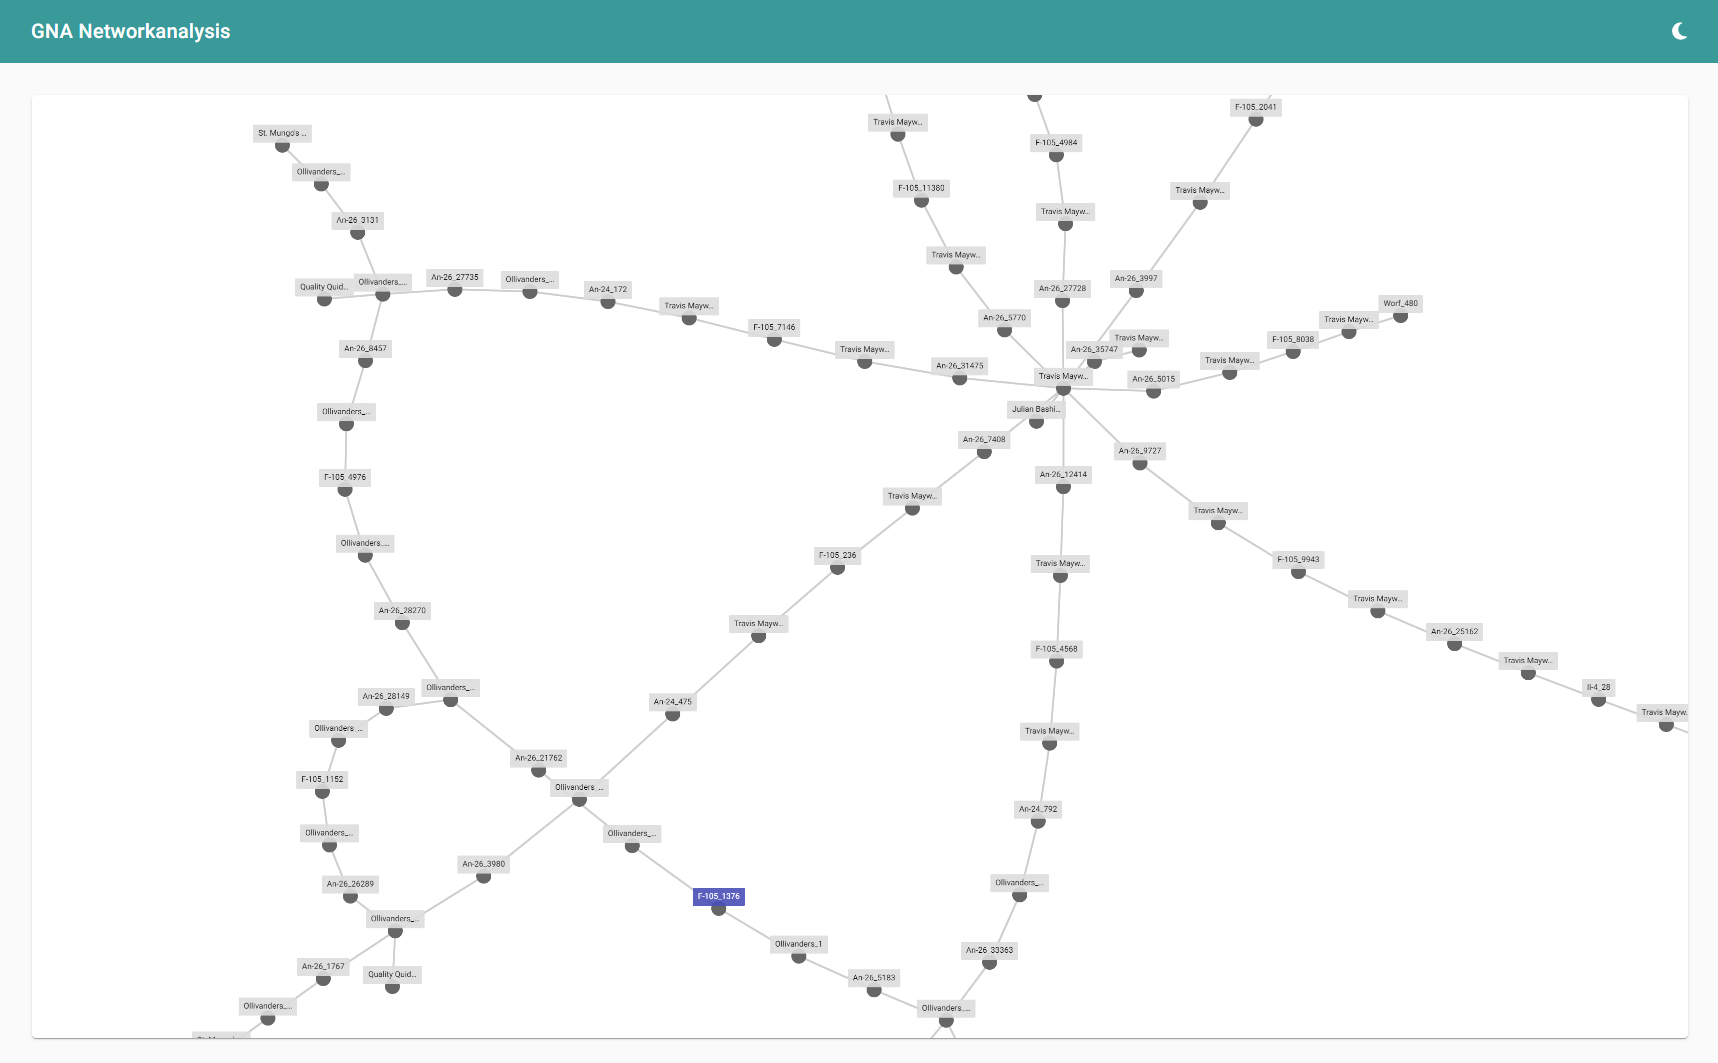
\includegraphics[width=1\textwidth]{content/img/Empire/Frontend/Angular_Graph_Prototype.png}
    \caption{Visualisierung eines Teils des Stromnetzwerkes in einem Graphen}
    \label{fig:AngularGraphPrototype}
\end{figure}
\FloatBarrier

Eine weitere Überlegung dieser Visualisierungsmethode ist der Einstiegspunkt beziehungsweise der Knoten, welcher als erstes geladen wird, gewesen. Denn aufgrund der schieren Menge an Elementen im Stromnetzwerk ist es einfach unmöglich alle Daten auf einmal zu laden. Aus diesem Grund wird immer nur ein Stück beziehungsweise ein kleiner Teil des Stromnetzwerkes angezeigt. Dabei ergibt sich jedoch die Frage: Welcher Teil des Netzwerks soll angezeigt werden, wenn nicht das gesamte Netzwerk angezeigt werden kann? Anders formuliert benötigen wir ein Startelement, von welchem aus die weiteren angeschlossenen Elemente geladen werden können. Somit haben wir die Möglichkeit, das Laden der Elemente auf eine gewisse Tiefe zu reduzieren. Folgendermaßen wird automatisch nur ein Teil des Graphen geladen, was wiederum die Schnelligkeit der Visualisierung deutlich erhöht.

Aus diesen genannten Gründen ist es bei unserer Applikation nicht möglich, den Graph ohne Startelement zu visualisieren. Und genau deswegen können Sie den Graphen auch nur ansehen, wenn Sie auf den \wordindoublequotes{Go to Graph →}-Button bei der Fehlertabelle klicken. Denn somit haben wir sichergestellt, dass der Graph mit einem fehlerhaften Objekt im Netzmodell startet, dessen nähere Umgebung Sie angenehm analysieren können. In Abbildung \ref{fig:AngularGraphCurrentErrorPrototype} können Sie sehr gut erkennen, dass das Startelement im Graphen auch blau markiert ist, damit die Siemens Ingenieure effizient und effektiv den Ursprung des Fehlers im Netzmodell ausfindig machen können.

\begin{figure}
    \centering
    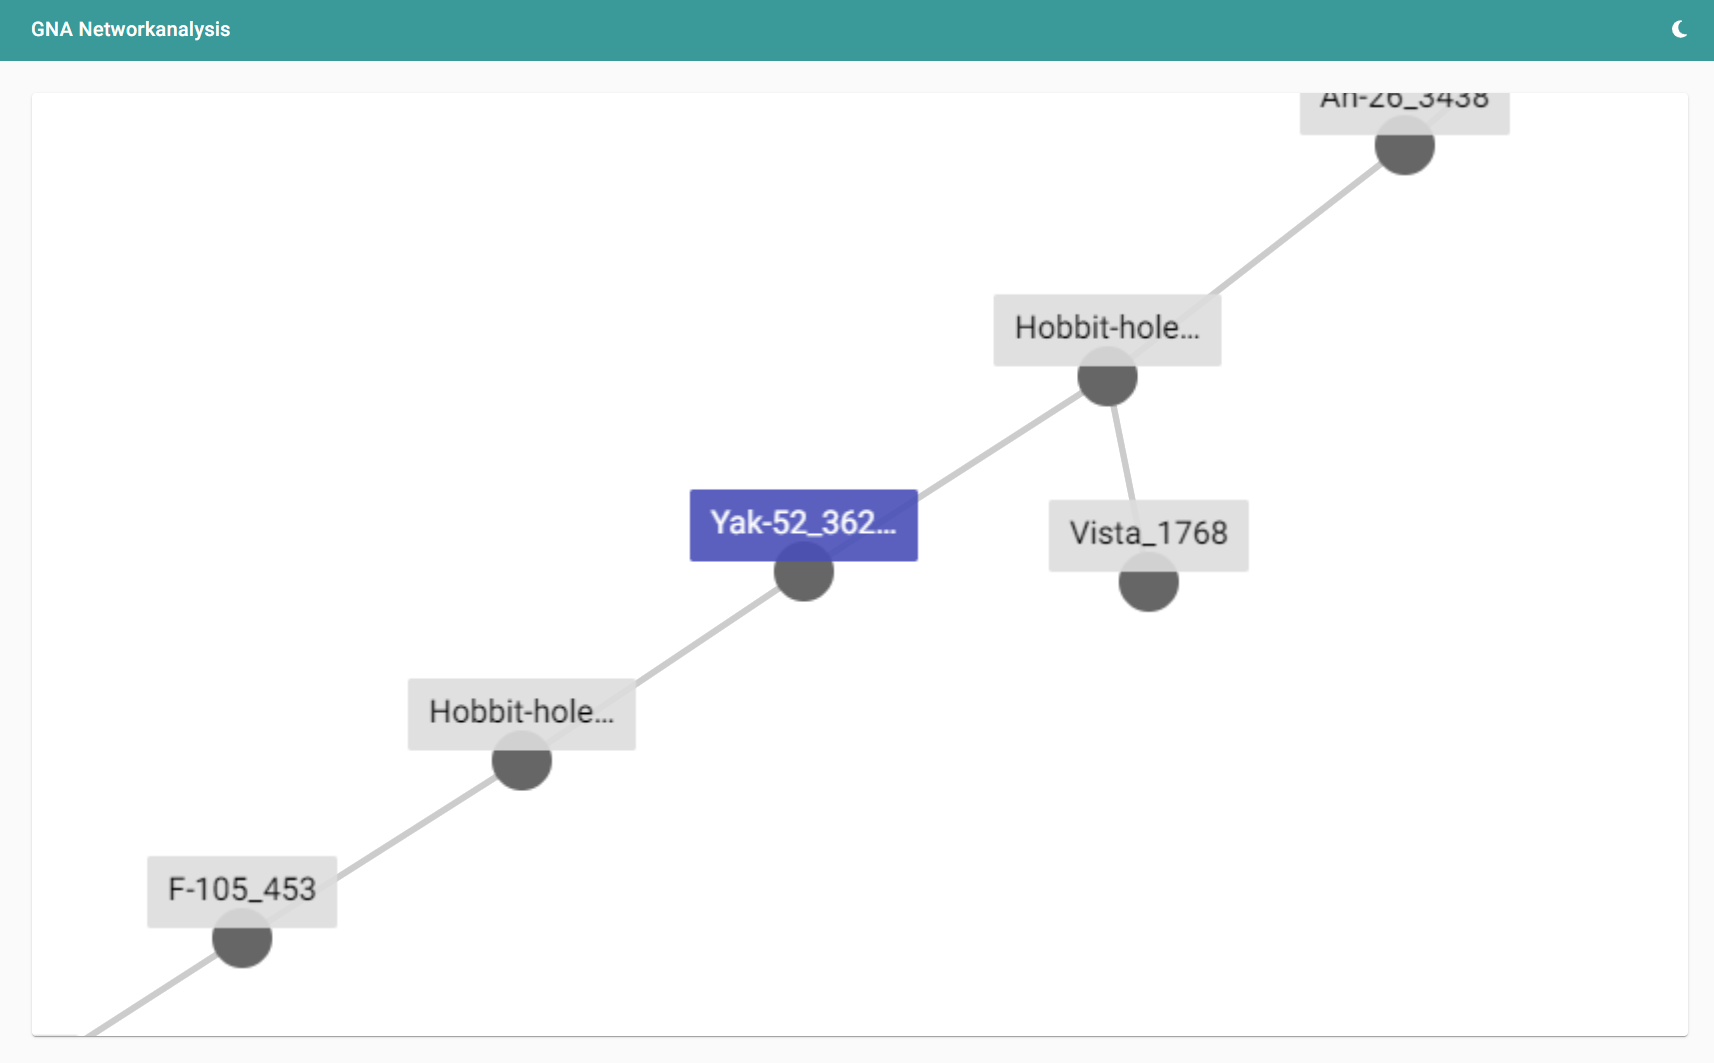
\includegraphics[width=1\textwidth]{content/img/Empire/Frontend/Angular_Graph_Current_Error_Prototype.png}
    \caption{Aktuelles fehlerhaftes Netzmodellobjekt im Graphen blau markiert}
    \label{fig:AngularGraphCurrentErrorPrototype}
\end{figure}
\FloatBarrier

In dieser Abbildung (\ref{fig:AngularGraphCurrentErrorPrototype}) sehen Sie auch trotz Anonymisierung der Daten, dass zwischen zwei aktiven Elementen (Schalter, Transformatoren, Widerstände, Generatoren, Sicherungen, usw.) meistens ein passives Element (hauptsächlich Leiter) liegt. Aktive Elemente beschreiben in dem Kontext eher Elemente, welche Eigenschaften des Stroms verändern, während passive diesen nur transportieren. Wie Sie sehen können, kommen diese beiden Gruppen -- aktive und passive Elemente -- abwechselnd hintereinander im Netzmodell vor: \wordindoublequotes{Hobbit-hole} -- \wordindoublequotes{Yak-52} -- \wordindoublequotes{Hobbit-hole}. Noch besser ist diese besondere Eigenschaft im Abbildung \ref{fig:AngularGraphAlternatingElementsPrototype} zu erkennen, wo sich \wordindoublequotes{Yak} und \wordindoublequotes{Dori} alternierend entlang der gelb markieren Verbindung ergänzen.

\setcapindent{90pt}
\begin{figure}
    \centering
    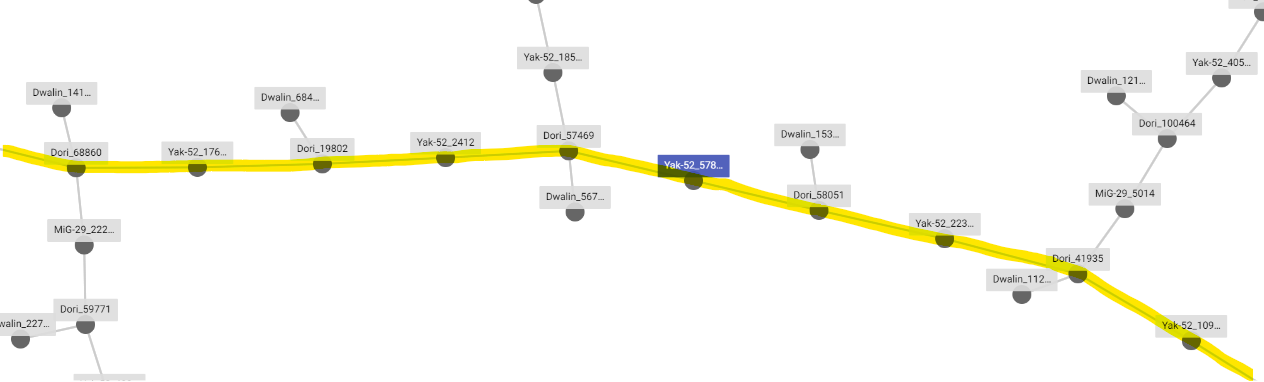
\includegraphics[width=1\textwidth]{content/img/Empire/Frontend/Angular_Graph_Alternating_Elements_Prototype.png}
    \caption{Abwechselnde Vorkommnis der verschiedenen Elementgruppen im Stromnetzwerk}
    \label{fig:AngularGraphAlternatingElementsPrototype}
\end{figure}
\FloatBarrier

Im Sinne des Graphen ist auch anzumerken, dass die Positionierung der Knoten keine geografische Bedeutung haben, da uns diese Art von topografischen Daten nicht zur Verfügung steht. Stattdessen werden die Knoten mithilfe des \emph{cola}-Layouts möglichst effizient angeordnet. Effizienz in diesem Sinne bedeutet, dass sich die Knoten, wären sie Atome, in einer möglichst ruhigen, entspannten Position und angenehmen Entfernung von anderen Knoten befinden. Dieses Layout unterstützt dementsprechend die Darstellung eines natürlichen biologischen Systems, da sich beispielsweise auch Zellen im menschlichen Körper gleichmäßig in den Blutbahnen verteilen. 
\section{Applikation im Dark Mode}

Zu guter Letzt sehen wir uns noch die Applikation im Dark Mode an. Diese Funktionalität ist meiner Meinung nach bei fast allen Webanwendungen ein Muss und genau aus diesem Grund wird sie logischerweise auch bei unserer Webapplikation unterstützt. Dank Angular in Kombination mit Angular Material ist die Umsetzung eines dunklen Modus wirklich nicht schwierig und zieht sich konsistent durch das gesamte Design durch. Dabei ist natürlich wichtig, dass die \emph{Corporate Identity} von Siemens nicht verloren geht, weshalb die Hauptfarbe wieder das ikonische Türkis ist. In den folgenden Abbildungen \ref{fig:AngularDashboardPrototypeDark}, \ref{fig:AngularFindingsPrototypeDark} und \ref{fig:AngularGraphPrototypeDark} können Sie Ihre Blicke über den angenehm zu erblickenden Dark Mode ruhen lassen.

\begin{figure}
    \centering
    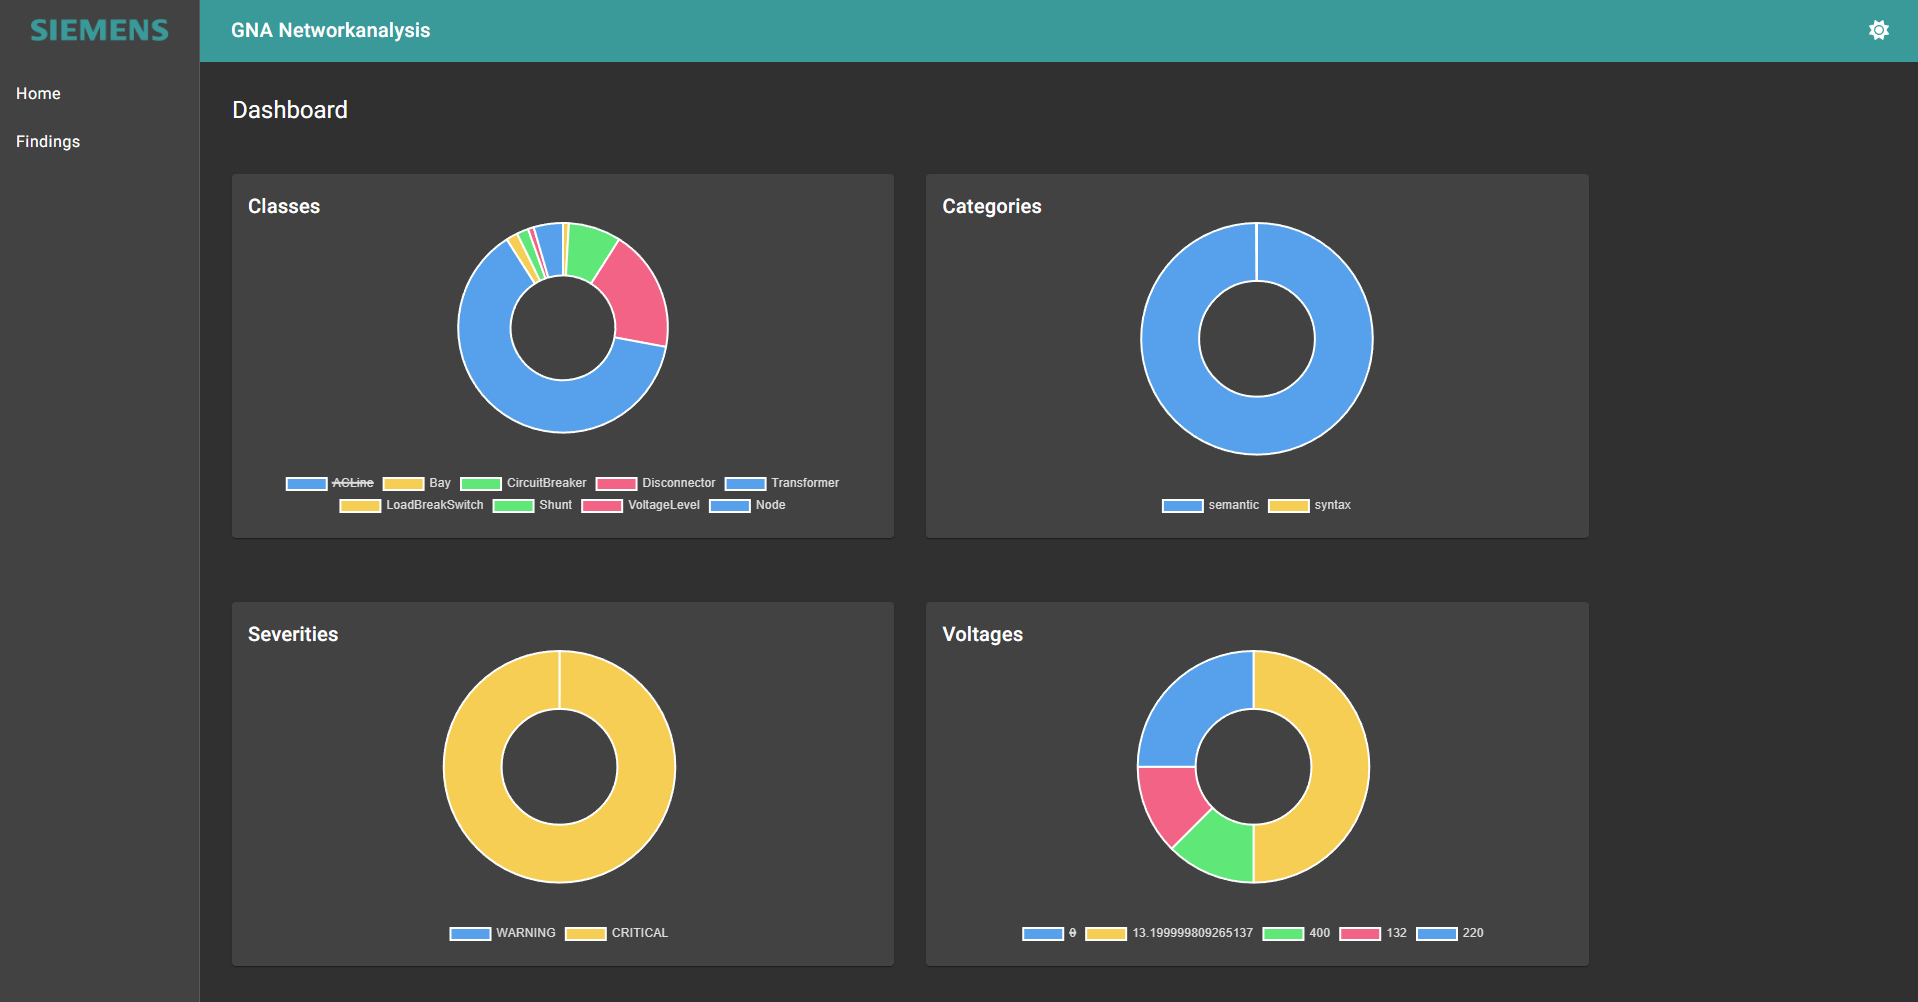
\includegraphics[width=1\textwidth]{content/img/Empire/Frontend/Angular_Dashboard_Prototype_Dark.png}
    \caption{Dashboard im Dark Mode}
    \label{fig:AngularDashboardPrototypeDark}
\end{figure}
\FloatBarrier

\begin{figure}
    \centering
    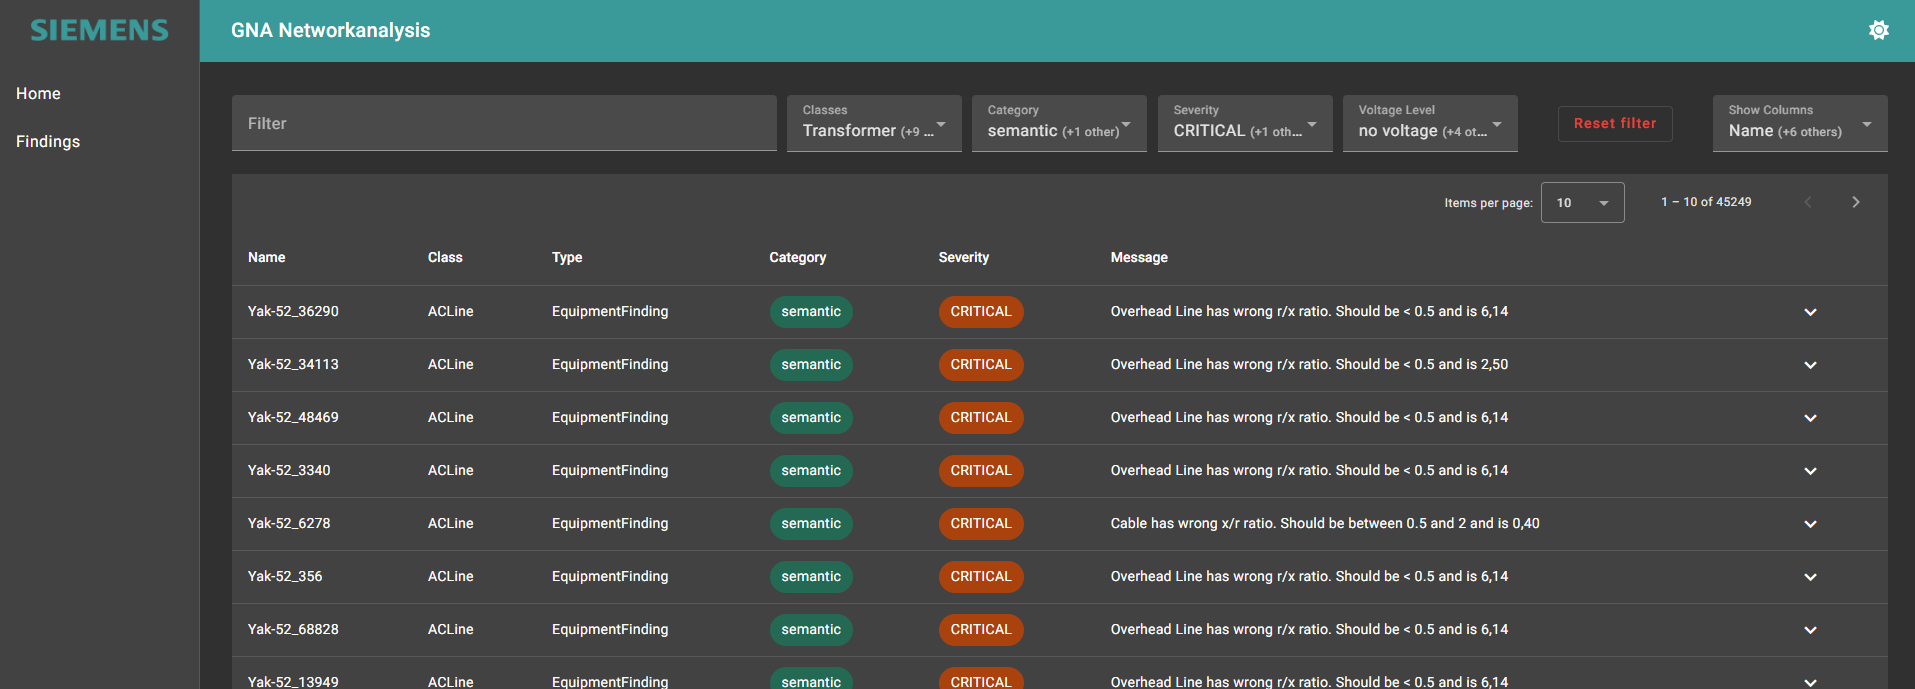
\includegraphics[width=1\textwidth]{content/img/Empire/Frontend/Angular_Findings_Prototype_Dark.png}
    \caption{Ergebnisse des Netzmodells im Dark Mode}
    \label{fig:AngularFindingsPrototypeDark}
\end{figure}
\FloatBarrier

\begin{figure}
    \centering
    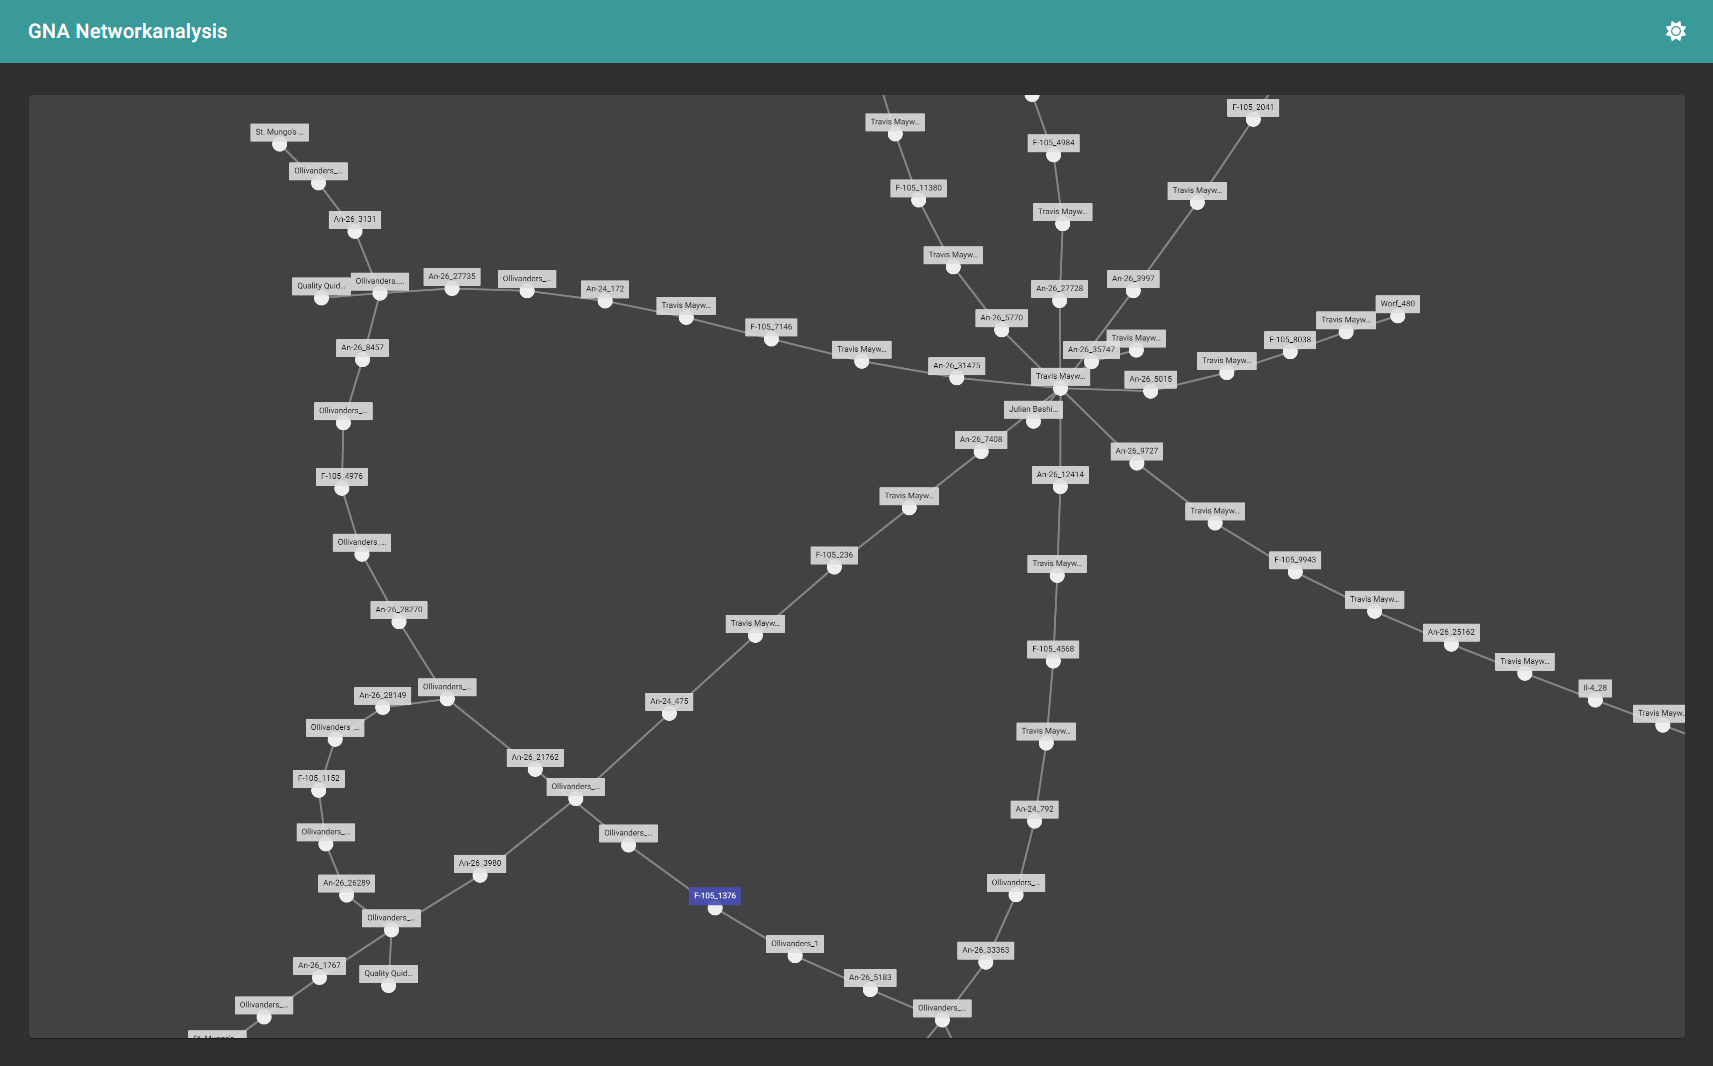
\includegraphics[width=1\textwidth]{content/img/Empire/Frontend/Angular_Graph_Prototype_Dark.png}
    \caption{Visualisierung des Stromnetzmodells mittels Graph im Dark Mode}
    \label{fig:AngularGraphPrototypeDark}
\end{figure}
\FloatBarrier